\chapter{Analiză și fundamentare teoretică}
\label{ch:analysis}
\pagestyle{fancy}

{\color{blue}Împreună cu \textbf{următoarele} 2 capitole trebuie să reprezinte aproximativ 70\% din total.\\}

Scopul acestui capitol este de a explica principiile funcționale ale aplicației implementate.
Aici se va descrie soluția propusă dintr-un punct de vedere teoretic - explicați și demonstrați proprietățile și valoarea teoretică:
\begin{itemize}
	\item algoritm utilizat sau propus
	\item protocoale utilizate
	\item modele abstracte
	\item explicații/argumentări logice ale soluției alese
	\item structura logică și funcțională a aplicației.
\end{itemize}


~\\\parbox[c]{\textwidth}{\color{red}\bfseries

NU SE FAC referiri la implementarea propriu-zisă.

NU SE PUN descrieri de tehnologii preluate cu copy-paste din alte surse sau lucruri care nu țin strict de proiectul propriu-zis (materiale de umplutură).
}

\section{Nume de secțiune}\label{sec:context}

\subsection{Nume de subsecțiune}\label{subsec:numesub}

Fiecare tabel introdus în lucrare este numerotat astfel: Tabel x.y, unde x reprezintă numărul capitolului, iar y numărul tabelului din capitol.
Se lasă un rând liber între tabel și paragraful anterior, respectiv posterior (tabelul~\ref{tab:nonlin}).

\begin{table}[ht]
    \caption{Rezultate}
    \centering                          % tabel centrat
    \begin{tabular}{|c|c|c|c|}          % 4 coloane centrate
        \hline
        Case & Method\#1 & Method\#2 & Method\#3 \\ [0.5ex]   % inserare tabel
        %heading
        \hline                              % linie orizontal simpla
        1 & 50 & 837 & 970 \\               % corpul tabelului
        2 & 47 & 877 & 230 \\
        3 & 31 & 25 & 415 \\[1ex]           % [1ex] adds vertical space
        \hline
    \end{tabular}
    % titlul tabelului
    \label{tab:nonlin}                % eticheta folosita pentru referirea tabelului in text; referirea in text se va face cu \ref{table:nonlin}
\end{table}


Fiecare figură introdusă în text este citată (de ex: în figura x.y este prezentată ...) și numerotată.
Numerotarea se face astfel Figura x.y unde x reprezintă numărul capitolului iar y numărul figurii în acel capitol.
Numerotarea o face automat latex pe baza etichetei (\verb+\label{}+).

Referirea unei figuri se face cu \verb+\ref{}+. De exemplu, referința: figura~\ref{fig:imag}.

\begin{figure}[ht]
    \centering
    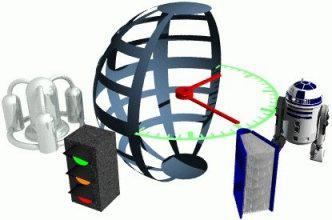
\includegraphics[]{figs/test.jpg}
    \caption{Numele figurii}
    \label{fig:imag}
\end{figure}

